%%
% This is an Overleaf template for presentations
% using the TUM Corporate Desing https://www.tum.de/cd
%
% For further details on how to use the template, take a look at our
% GitLab repository and browse through our test documents
% https://gitlab.lrz.de/latex4ei/tum-templates.
%
% The tumbeamer class is based on the beamer class.
% If you need further customization please consult the beamer class guide
% https://ctan.org/pkg/beamer.
% Additional class options are passed down to the base class.
%
% If you encounter any bugs or undesired behaviour, please raise an issue
% in our GitLab repository
% https://gitlab.lrz.de/latex4ei/tum-templates/issues
% and provide a description and minimal working example of your problem.
%%

\documentclass[
  german,            % define the document language (english, german)
  aspectratio=169,    % define the aspect ratio (169, 43)
  % handout=2on1,       % create handout with multiple slides (2on1, 4on1)
  % partpage=false,     % insert page at beginning of parts (true, false)
  % sectionpage=true,   % insert page at beginning of sections (true, false)
]{tumbeamer}

 
% load additional packages

\usepackage{graphicx}
\usepackage{tikz}
\usepackage{url}
\usepackage{pgfplots}
\usepackage{hyperref}
\usepackage{pmboxdraw}
\usepackage{float}
\usepackage{babel}[ngerman]
\usepackage{csquotes}[autostyle]
\usepackage[useregional]{datetime2}
\usepackage{listings}
\usepackage{xurl}
\usepackage{enumerate}
\usepackage{circuitikz}
\usepackage{csquotes}
\usepackage{tikz-timing}
\usepackage{colortbl}
\usepackage{ifthen}
\usepackage{ulem}
\usepackage{pgf}
\usepackage{amsmath}
\usepackage{amssymb}
\usepackage{xcolor}
\usepackage{karnaugh-map}

% \usepackage{minted}
% \usemintedstyle{borland}
\usetikzlibrary{patterns}
\pgfplotsset{compat=1.18}

% tikz
\usetikzlibrary{overlay-beamer-styles}
\usetikzlibrary{arrows,backgrounds,positioning,shapes,,patterns,patterns.meta,matrix,arrows.meta,shapes.geometric}
\usetikzlibrary{matrix, fit, calc}
%\usetikzlibrary{automata}
% requires circuitikz >= 1.1.0
% for distros with older distributions, install TeX Live manually
% instead of using your package manager
% see: https://tug.org/texlive/quickinstall.html
\ctikzset{logic ports=european}

% minted
% \setminted{
%     fontsize=\small, 
%     frame=none,
%     breaklines=false,
% }

\lstset {
    frame=single,
    tabsize=4,
    breaklines=true,
    xleftmargin=5pt,
    xrightmargin=5pt,
    basicstyle=\ttfamily\footnotesize,
    %language=[RISC-V]Assembler,
}

\hypersetup { 
  colorlinks=true,
  urlcolor=blue,
  filecolor=black,
  linkcolor=black
}

% commands
\newcommand{\n}[1]{\overline{#1}}

% image path
\graphicspath{ {../resources/} }

% presentation metadata
\title{Übung 12: Optimierung}

\subtitle{Einführung in die Rechnerarchitektur}

\author{\theAuthorName}

\institute{\theGroupName\\\theSchoolName\\\theUniversityName}
\date{20. -- \DTMdisplaydate{2025}{01}{26}{-1}}

\footline{\insertauthor~|~\insertshorttitle~|~\insertshortdate}


% macro to configure the style of the presentation
\TUMbeamersetup{
  title page = TUM tower,         % style of the title page
  part page = TUM toc,            % style of part pages
  section page = TUM toc,         % style of section pages
  content page = TUM more space,  % style of normal content pages
  tower scale = 1.0,              % scaling factor of TUM tower (if used)
  headline = TUM threeliner,      % which variation of headline to use
  footline = TUM default,         % which variation of footline to use
  % configure on which pages headlines and footlines should be printed
  headline on = {title page},
  footline on = {every page, title page=false},
}


% available frame styles for title page, part page, and section page:
% TUM default, TUM tower, TUM centered,
% TUM blue default, TUM blue tower, TUM blue centered,
% TUM shaded default, TUM shaded tower, TUM shaded centered,
% TUM flags
%
% additional frame styles for part page and section page:
% TUM toc
%
% available frame styles for content pages:
% TUM default, TUM more space
%
% available headline options:
% TUM empty, TUM oneliner, TUM twoliner, TUM threeliner, TUM logothreeliner
%
% available footline options:
% TUM empty, TUM default, TUM infoline

\begin{document}

\maketitle

\begin{frame}[c]{Mitschriften \& Infos}{}
  \begin{minipage}[t]{\textwidth}
    \begin{columns}[c]
      \begin{column}{0.8\textwidth}
        Montags: \href{\zulipMo}{\zulipMo}
      \end{column}
      \begin{column}{0.2\textwidth}
        \includegraphics[width=0.8\linewidth]{\zulipMoQrFilename}
      \end{column}
    \end{columns}
  \end{minipage}
  \rule{\textwidth}{0.4pt}
  \begin{minipage}[t]{\textwidth}
    \begin{columns}[c]
      \begin{column}{0.8\textwidth}
        Donnerstags: \href{\zulipDo}{\zulipDo}
      \end{column}
      \begin{column}{0.2\textwidth}
        \includegraphics[width=0.8\linewidth]{\zulipDoQrFilename}
      \end{column}
    \end{columns}
  \end{minipage}
  \ifdefined\myWebsite
  \rule{\textwidth}{0.4pt}
  \centering
  Website: \href{\myWebsite}{\myWebsite}
  \fi
\end{frame}

\begin{frame}[c]{}{}
  \begin{center}
    \LARGE  Keine Garantie für die Richtigkeit der Tutorfolien.

    \Large Bei Unklarheiten/Unstimmigkeiten haben VL/ZÜ-Folien recht!
  \end{center}
\end{frame}

\begin{frame}[c]{Inhaltsübersicht}{}
  \begin{columns}[c]
    \begin{column}{1\textwidth}
      \begin{itemize}
        \item Quiz
        \item Wiederholung
        \item Tutorblatt
        \begin{itemize}
			\item Sieben-Segment-Anzeige (KV-Maps)
			\item Logik-Hazards
			\item BDD Reduktion
			\item Konstruktion von BDDs
        \end{itemize}
      \end{itemize}
    \end{column}
  \end{columns}
\end{frame}

\begin{frame}[fragile, c]{Logiksynthese}{}
	\begin{itemize}
		\item Realisierung: boolsche Funktion $\rightarrow$ Schaltung
		\item naive Synthese (direkte Übertragung der Wahrheitstabelle) nicht skalierbar
		\item verschiedene Verfahren zur Optimierung und Reduktion von Funktionen auf ihr Minimalpolynom
	\end{itemize}
	\begin{block}{Minimalpolynom}
		Ein Polynom $p$ ist Minimalpolynom einer booleschen Funktion $f$, falls  $\psi(p) \equiv f$ (d.h. $p$ eine Formel für $f$ ist) und es keine weitere Vereinfachungen gibt.
	\end{block}
\end{frame}

\begin{frame}[fragile, c]{Karnaugh-Veitch-Diagramme\footnote{Oft auch als K-Maps bezeichnet}}{}
\begin{columns}[c]
\begin{column}{0.6\textwidth}
	\begin{itemize}
		\item rechteckiges Schema, in dem alle Literalkombinationen (positiv und negativ) vorkommen
		\item nebeneinander liegende Zeilen/Spalten dürfen sich immer nur in 1 Bit unterscheiden (Gray-Code)!
		\item Zusammenfassen von Einsen in $2^n$-Blöcken. Don't Care können als $0$ oder $1$ gewählt werden.
		\item Jedes maximal große Päckchen steht für einen Primimplikanten der Funktion $\rightarrow$ alle Päckchen zusammen ergeben ein Minimalpolynom

	\end{itemize}
\end{column}
\begin{column}{0.4\textwidth}
\begin{center}
\resizebox{!}{0.6\textheight}{
	\begin{karnaugh-map}(label=corner,implicantcolors={red,lime,orange,blue,violet})[4][4][1][B][A][D][C]
	\maxterms{3,6,7,12,9} % zeroes
	\minterms{4,5,15,14,8,11,10,13,2} % ones
	\implicant{0}{5}
	\implicant{15}{10}
	\implicant{5}{13}
	\implicantcorner
	\autoterms[-]
	\end{karnaugh-map}
}\\
$f=\textcolor{red}{\bar a\bar c}+\textcolor{blue}{\bar b\bar d}+\textcolor{lime}{ac} +\textcolor{orange}{\bar abd}$
\end{center}
\end{column}
\end{columns}

\end{frame}


\begin{frame}[fragile, c]{Logik-Hazads}{}
	\begin{columns}[c]
	\begin{column}{0.5\textwidth}
		\begin{itemize}
			\item Änderung eines Eingangs ändert kurzzeitig Ausgang, obwohl nach den Regeln der	Booleschen Algebra keine Änderung auftritt
			\item Kann bei sequenziellen Schaltungen problematisch werden (z.B. Oszillation)
			\item Beispiel
			\begin{itemize}
				\item A=0, B=1, C=1 → Y = 1
				\item A=0, B=0, C=1 → Y = 1
			\end{itemize} 
		\end{itemize}
	\end{column}
	\begin{column}{0.5\textwidth}
	\begin{center}
	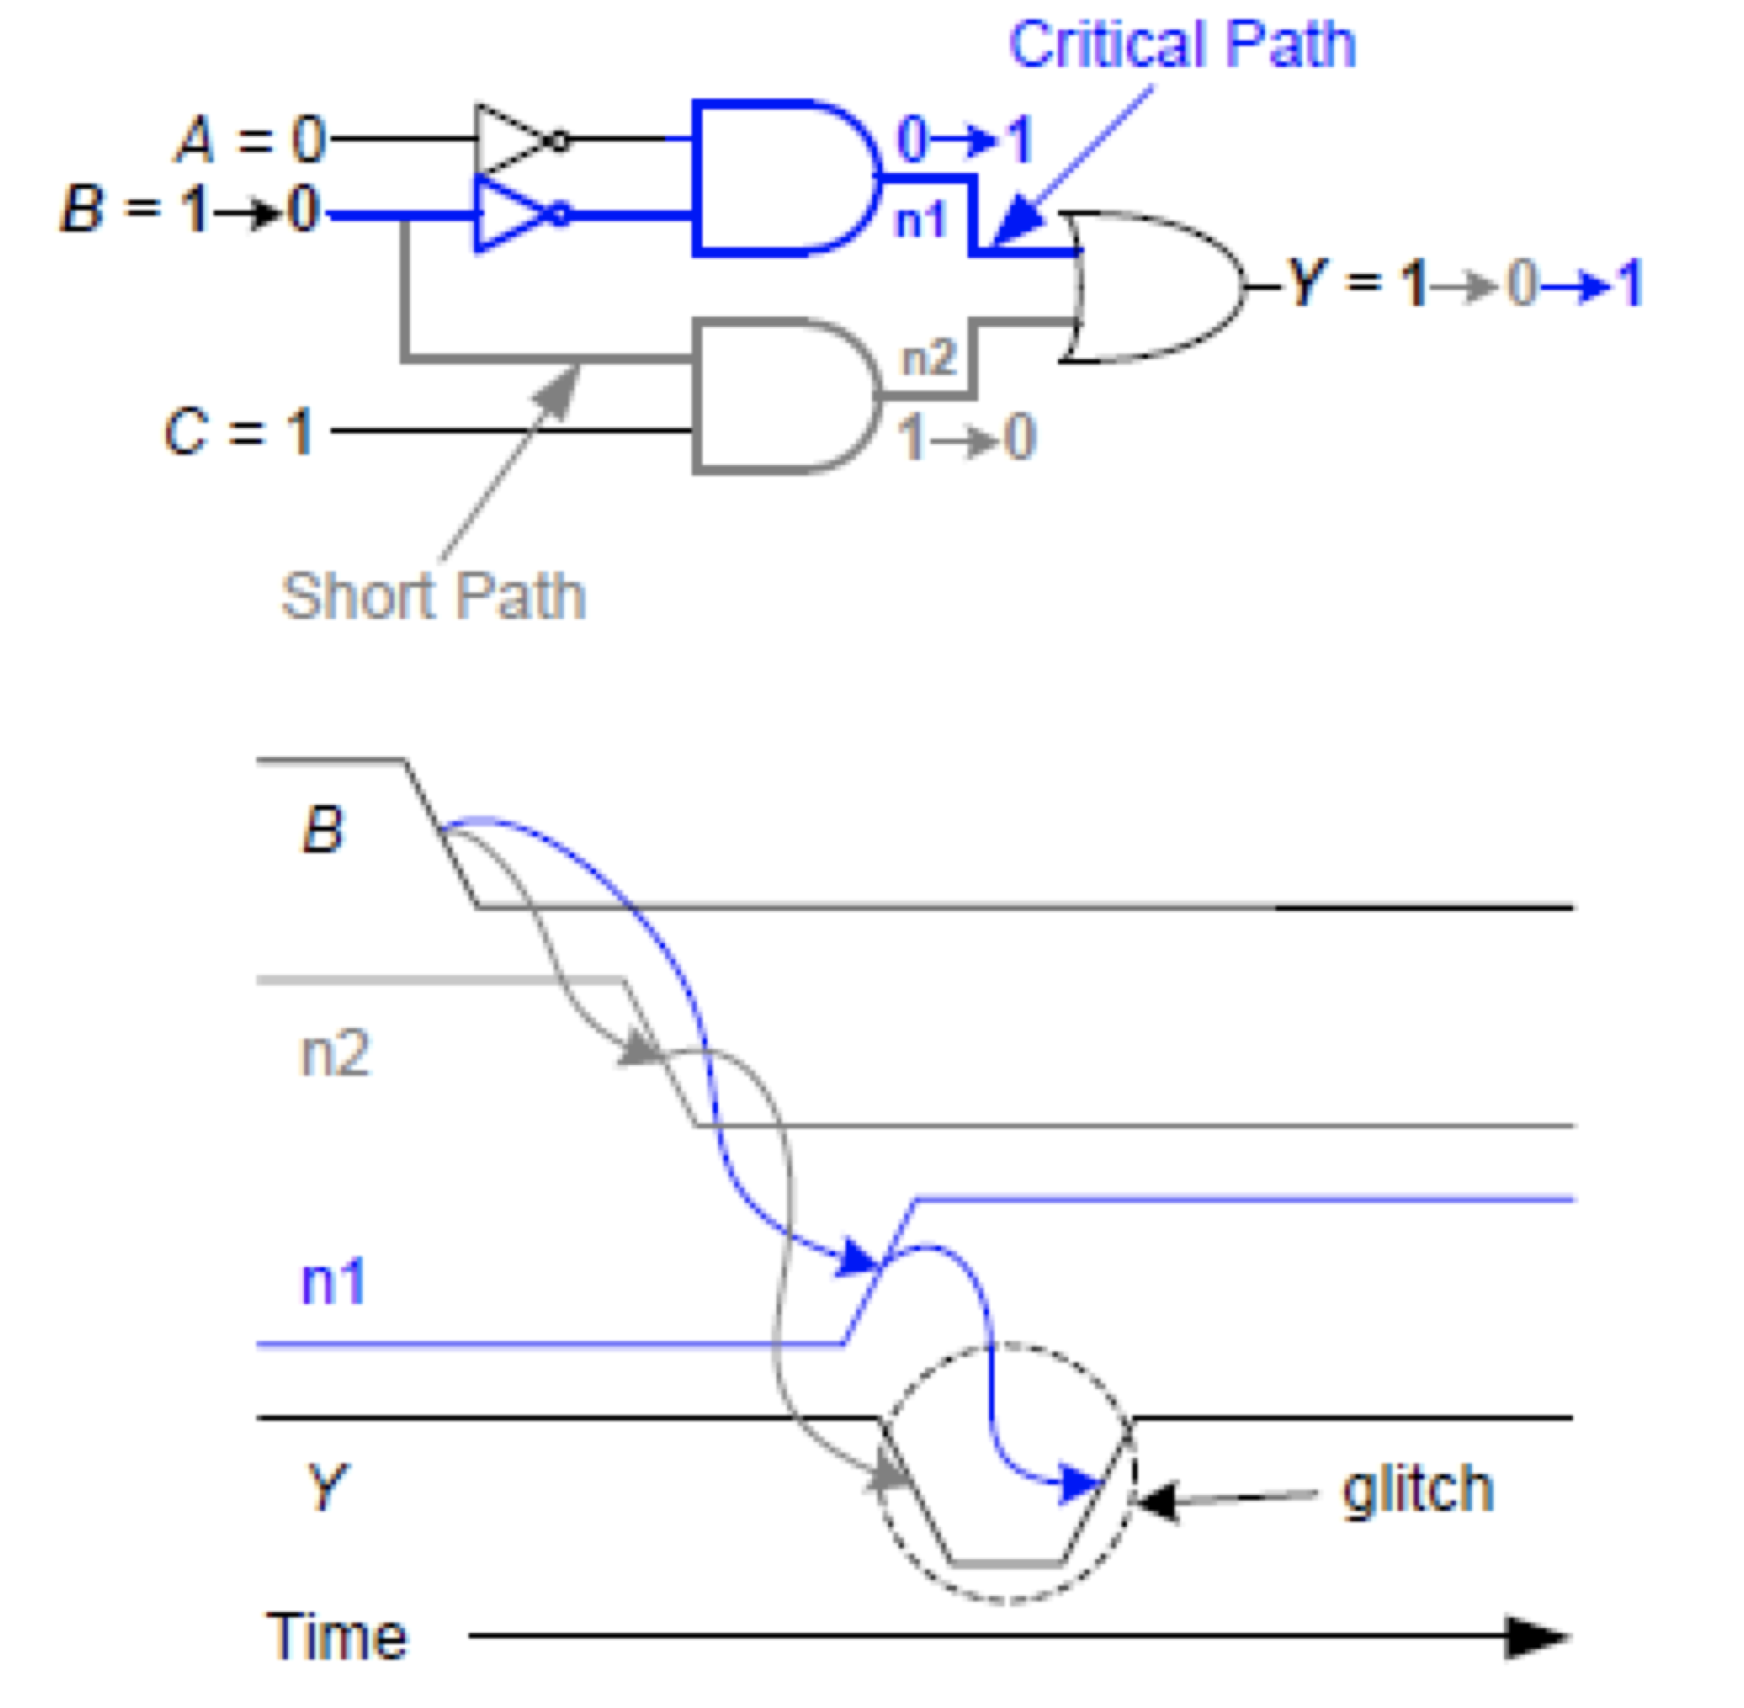
\includegraphics[width=0.9\textwidth]{w12_logik_hazard.png}
	\end{center}
	\end{column}
	\end{columns}
	
	\end{frame}

% stolen from sheet u12
\tikzset{
	zeroarrow/.style = {-stealth,dashed},
	onearrow/.style = {-stealth,solid},
	c/.style = {circle,draw,solid,minimum width=2em,
		minimum height=2em},
	r/.style = {rectangle,draw,solid,minimum width=2em,
		minimum height=2em},
	e/.style = {draw=none,circle, minimum width=2em,minimum height=2em}
}
\begin{frame}[c, fragile]{Binary Decision Diagrams (BDDs)}{}
	\begin{columns}[c]
		\begin{column}{0.5\textwidth}
			\begin{itemize}
				\item Darstellung einer boolschen Funktion als gerichteter azyklischer Graph (DAG)
				\item Knoten repräsentieren Teilfunktionen, 2 ausgehende Kanten: $0, 1$
				\item Aufbau bspw. mittels Shannon-Zerlegung: $f(x_0, x_1) \rightarrow f_{x_0=0}(x_1), f_{x_0=1}(x_1)$
				\item ROBDDs sind kanonisch (eindeutig)!
			\end{itemize}
		\end{column}
		\begin{column}{0.5\textwidth}
			 \begin{center}
			 	\resizebox{!}{0.8\textheight}{
				\begin{tikzpicture}[node distance=1cm and 1cm]\footnotesize
					\node[c] (x1) {$x_1$};
					\node[] (t) [above=of x1, yshift=-0.8cm] {$\n{x}_1x_2\n{x}_3+x_1\n{x}_2\n{x}_3+x_1x_2x_3$};
					\node[c] (x2l) [below left=of x1] {$x_2$};
					\node[c] (x2r) [below right=of x1] {$x_2$};
					
					\node[c] (x3l) [below=of x2l] {$x_3$};
					\node[c] (x3r) [below=of x2r] {$x_3$};
					
					\node[r] (zero) [below=of x3r, xshift=-0.5cm] {0};
					\node[r] (one) [below=of x3l, xshift=0.5cm] {1};

					\draw[zeroarrow] (x1) -- (x2l) node [midway, fill=none, above left] {$x_2\n{x}_3$};
					\draw[onearrow] (x1) -- (x2r)  node [near end, fill=none, above right, align=center] {$\n{x}_2\n{x}_3+$\\$x_2x_3$};
					
					\draw[zeroarrow] (x2l) to [out=0,in=180] (zero);
					\draw[onearrow] (x2l) -- (x3l) node [midway, fill=none, left] {$\n{x}_3$};
	
					\draw[zeroarrow] (x2r) -- (x3l)  node [near end, fill=none, above left] {$\n{x}_3$};
					\draw[onearrow] (x2r)  -- (x3r)  node [midway, fill=none,right] {$x_3$};
					
					\draw[zeroarrow] (x3l) -- (one);
					\draw[onearrow] (x3l) -- (zero);
					\draw[zeroarrow] (x3r) -- (zero);
					\draw[onearrow] (x3r) -- (one);
				\end{tikzpicture}
			}\\
		\scriptsize Variablenordnung: $x_1\prec x_2\prec x_3$
			\end{center}
		\end{column}
	\end{columns}

\end{frame}

\begin{frame}[c, fragile]{BDDs: Reduktionen}
	\begin{columns}[c]
	\begin{column}{0.5\textwidth}
		\begin{center}
			\textbf{I-Reduktion}\\
			Zusammenführung isomorpher Knoten
			\vspace{\baselineskip}
			\resizebox{!}{0.5\textheight}{
			\begin{tikzpicture}
				\node[e] (rl) {};
				\node[e] (rm) [right=1em of rl]{};
				\node[e] (rr) [right=1em of rm]{};
				\node[c] (al) [below=of rl] {$a$};
				\node[c] (ar) [below=of rr] {$a$};
				
				\node[c] (bl) [below=of al] {$b$};
				\node[c] (br) [below=of ar] {$b$};
				
				\draw[zeroarrow] (rl) -- (al);
				\draw[zeroarrow] (rm) -- (ar);
				\draw[onearrow] (rr) -- (ar);
				
				\draw[zeroarrow] (al) -- (bl);
				\draw[zeroarrow] (ar) -- (bl);
				
				\draw[onearrow] (al) -- (br);
				\draw[onearrow] (ar) -- (br);
				
				\node[e] (rl2) [right=4em of rr]{};
				\node[e] (rm2) [right=1em of rl2]{};
				\node[e] (rr2) [right=1em of rm2]{};
				\node[c] (al2) [below=of rl2] {$a$};
				
				\node[c] (bl2) [below=of al2] {$b$};
				\node[c] (br2) [below=of al2, xshift=2cm] {$b$};
				
				\draw[zeroarrow] (rl2) -- (al2);
				\draw[zeroarrow] (rm2) -- (al2);
				\draw[onearrow] (rr2) -- (al2);
				
				\draw[zeroarrow] (al2) -- (bl2);
				\draw[zeroarrow] (al2) -- (bl2);
				
				\draw[onearrow] (al2) -- (br2);
				\draw[onearrow] (al2) -- (br2);
				
				\draw[->, very thick] (ar)++(2em,0) -- ++(2em,0);
		\end{tikzpicture}
	}
		\end{center}
	\end{column}
\begin{column}{0.5\textwidth}
	\begin{center}
		\textbf{S-Reduktion}\\
		Überflüssige Knoten entfernen
		\vspace{\baselineskip}
		\resizebox{!}{0.5\textheight}{
			\begin{tikzpicture}
				\node[e] (rl) {};
				\node[e] (rm) [right=1em of rl]{};
				\node[e] (rr) [right=1em of rm]{};
				\node[c] (al) [below=of rm] {$a$};
				\node[c] (bl) [below=of al] {$b$};
				
				\draw[zeroarrow] (rl) -- (al);
				\draw[zeroarrow] (rm) -- (al);
				\draw[onearrow] (rr) -- (al);
				
				\draw[zeroarrow] (al) to[bend right] (bl);
				\draw[onearrow] (al) to[bend left] (bl);
				
				\node[e] (rl2) [right=0em of rr]{};
				\node[e] (rm2) [right=1em of rl2]{};
				\node[e] (rr2) [right=1em of rm2]{};
	
				\node[e] (al2) [below=of rm2] {};
				\node[c] (bl2) [below=of al2] {$b$};
				
				\draw[zeroarrow] (rl2) -- (bl2);
				\draw[zeroarrow] (rm2) -- (bl2);
				\draw[onearrow] (rr2) -- (bl2);
				
				\draw[->, very thick] (al)++(3em,0) -- ++(2em,0);
			\end{tikzpicture}
		}
	\end{center}
\end{column}
\end{columns}
\end{frame}

\begin{frame}[c, fragile]{BDDs: Variablenordnungen}
	\begin{center}
		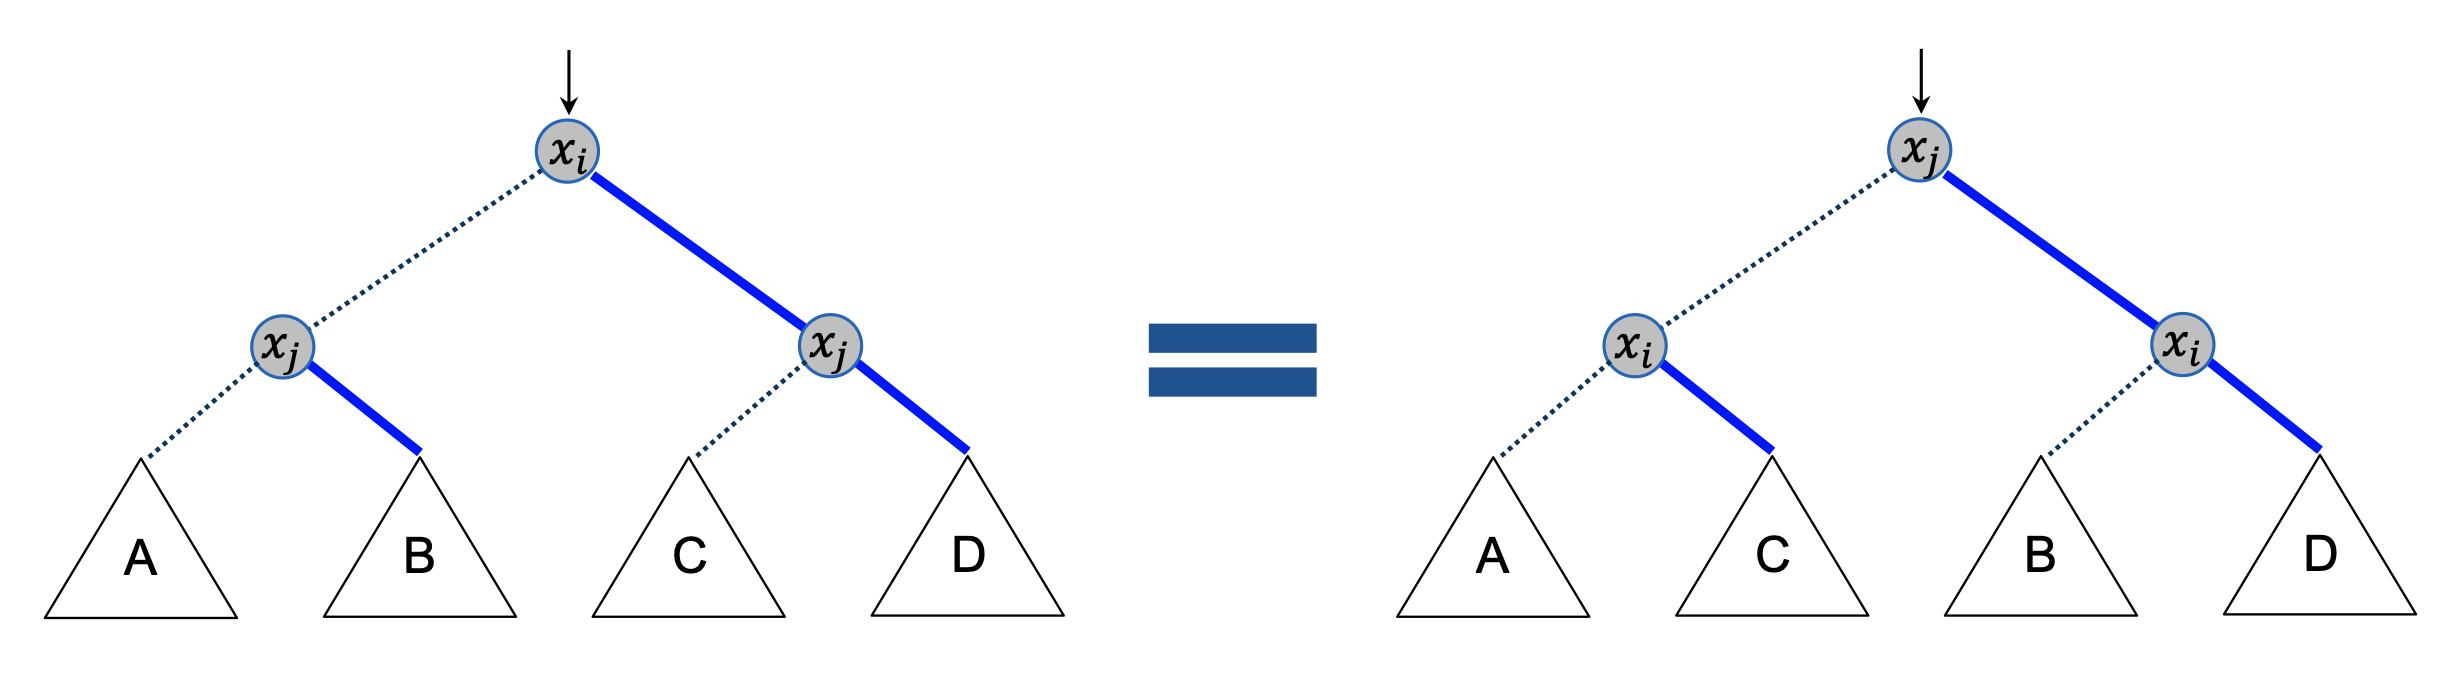
\includegraphics[width=0.8\textwidth]{w12_BDD_Variablenordnungen.png}
	\end{center}
	\begin{itemize}
		\item Vertauschen nur durch Ändern der Knotenanzahl und Umordnen der Kanten möglich
		\item Neue Reduktionsmöglichkeiten durch Vertauschen
		\item Finden einer guten Variablenordnung NP vollständig → Heuritische Lösungen
	\end{itemize}
\end{frame}

\begin{frame}[c]{Feedback}{} 
  \begin{center}
    \includegraphics[width=0.30\textwidth]{\myFeedbackQrFilename}
  \end{center}
  \begin{center}
    \LARGE \href{\myFeedbackLink}{\myFeedbackLink}
  \end{center}
  \vspace{0.5cm}
  \begin{center}
    \small Ein Teil der Folien stammt aus dem Foliensatz von Niklas Ladurner. Vielen Dank dafür!
  \end{center}
\end{frame}

\end{document}